
\subsection{Validation of the Restraint Selection Algorithm}
To assess the performance of the greedy algorithm for selecting optimal distance restraints between two molecules, it was first tested on toy models. These contained 12 to 30 particles that were randomly distributed in space. The particles were randomly assigned to two entities representing two molecules. A selection of four restraints was performed with no pre-processing steps. Different algorithmic approaches were compared: the developed greedy algorithm, an averaged random selection (100 repetitions), and two brute-force approaches. One of the brute-force approaches maximizes the sum of the restraint midpoint distances between the selected restraints by considering all possible quadruples of restraints explicitly (BF-maxD). The other one maximizes the CHV around the selected restraints (BF-maxCHV), as done for chaining in multi-state systems. Each number of particles was sampled 20 times (using different particle coordinates each time) to provide an uncertainty estimate. The scripts for this validation are available in the example folder of the GitHub repository (\textit{examples/publication/a\_benchmark\_algorithms}).

\subsection{Molecules with Hydration Free Energies}
The algorithm was applied for the calculation of relative hydration free energies $\Delta \Delta G_{\text{hyd}}$ (Figure \ref{fig:thermodynamic_cycle}).
A set of 16 molecules with experimentally available hydration free energies\cite{Wolfenden1987,Rizzo2006,Nicholls2008,Guthrie2009,Guthrie2014,Mobley2014} were selected (Table \ref{tab:SI_moleculelist}). 
The topologies for these molecules were taken from the ATB server.\cite{Stroet2018} The selected molecules are small and possess a ring core. The corresponding pairwise transformations are nevertheless relatively complex, and involve R-group and ring-size changes as well as scaffold hopping-type transformations (e.g. benzene to cyclohexane).

\begin{figure}[h!]
    \centering
    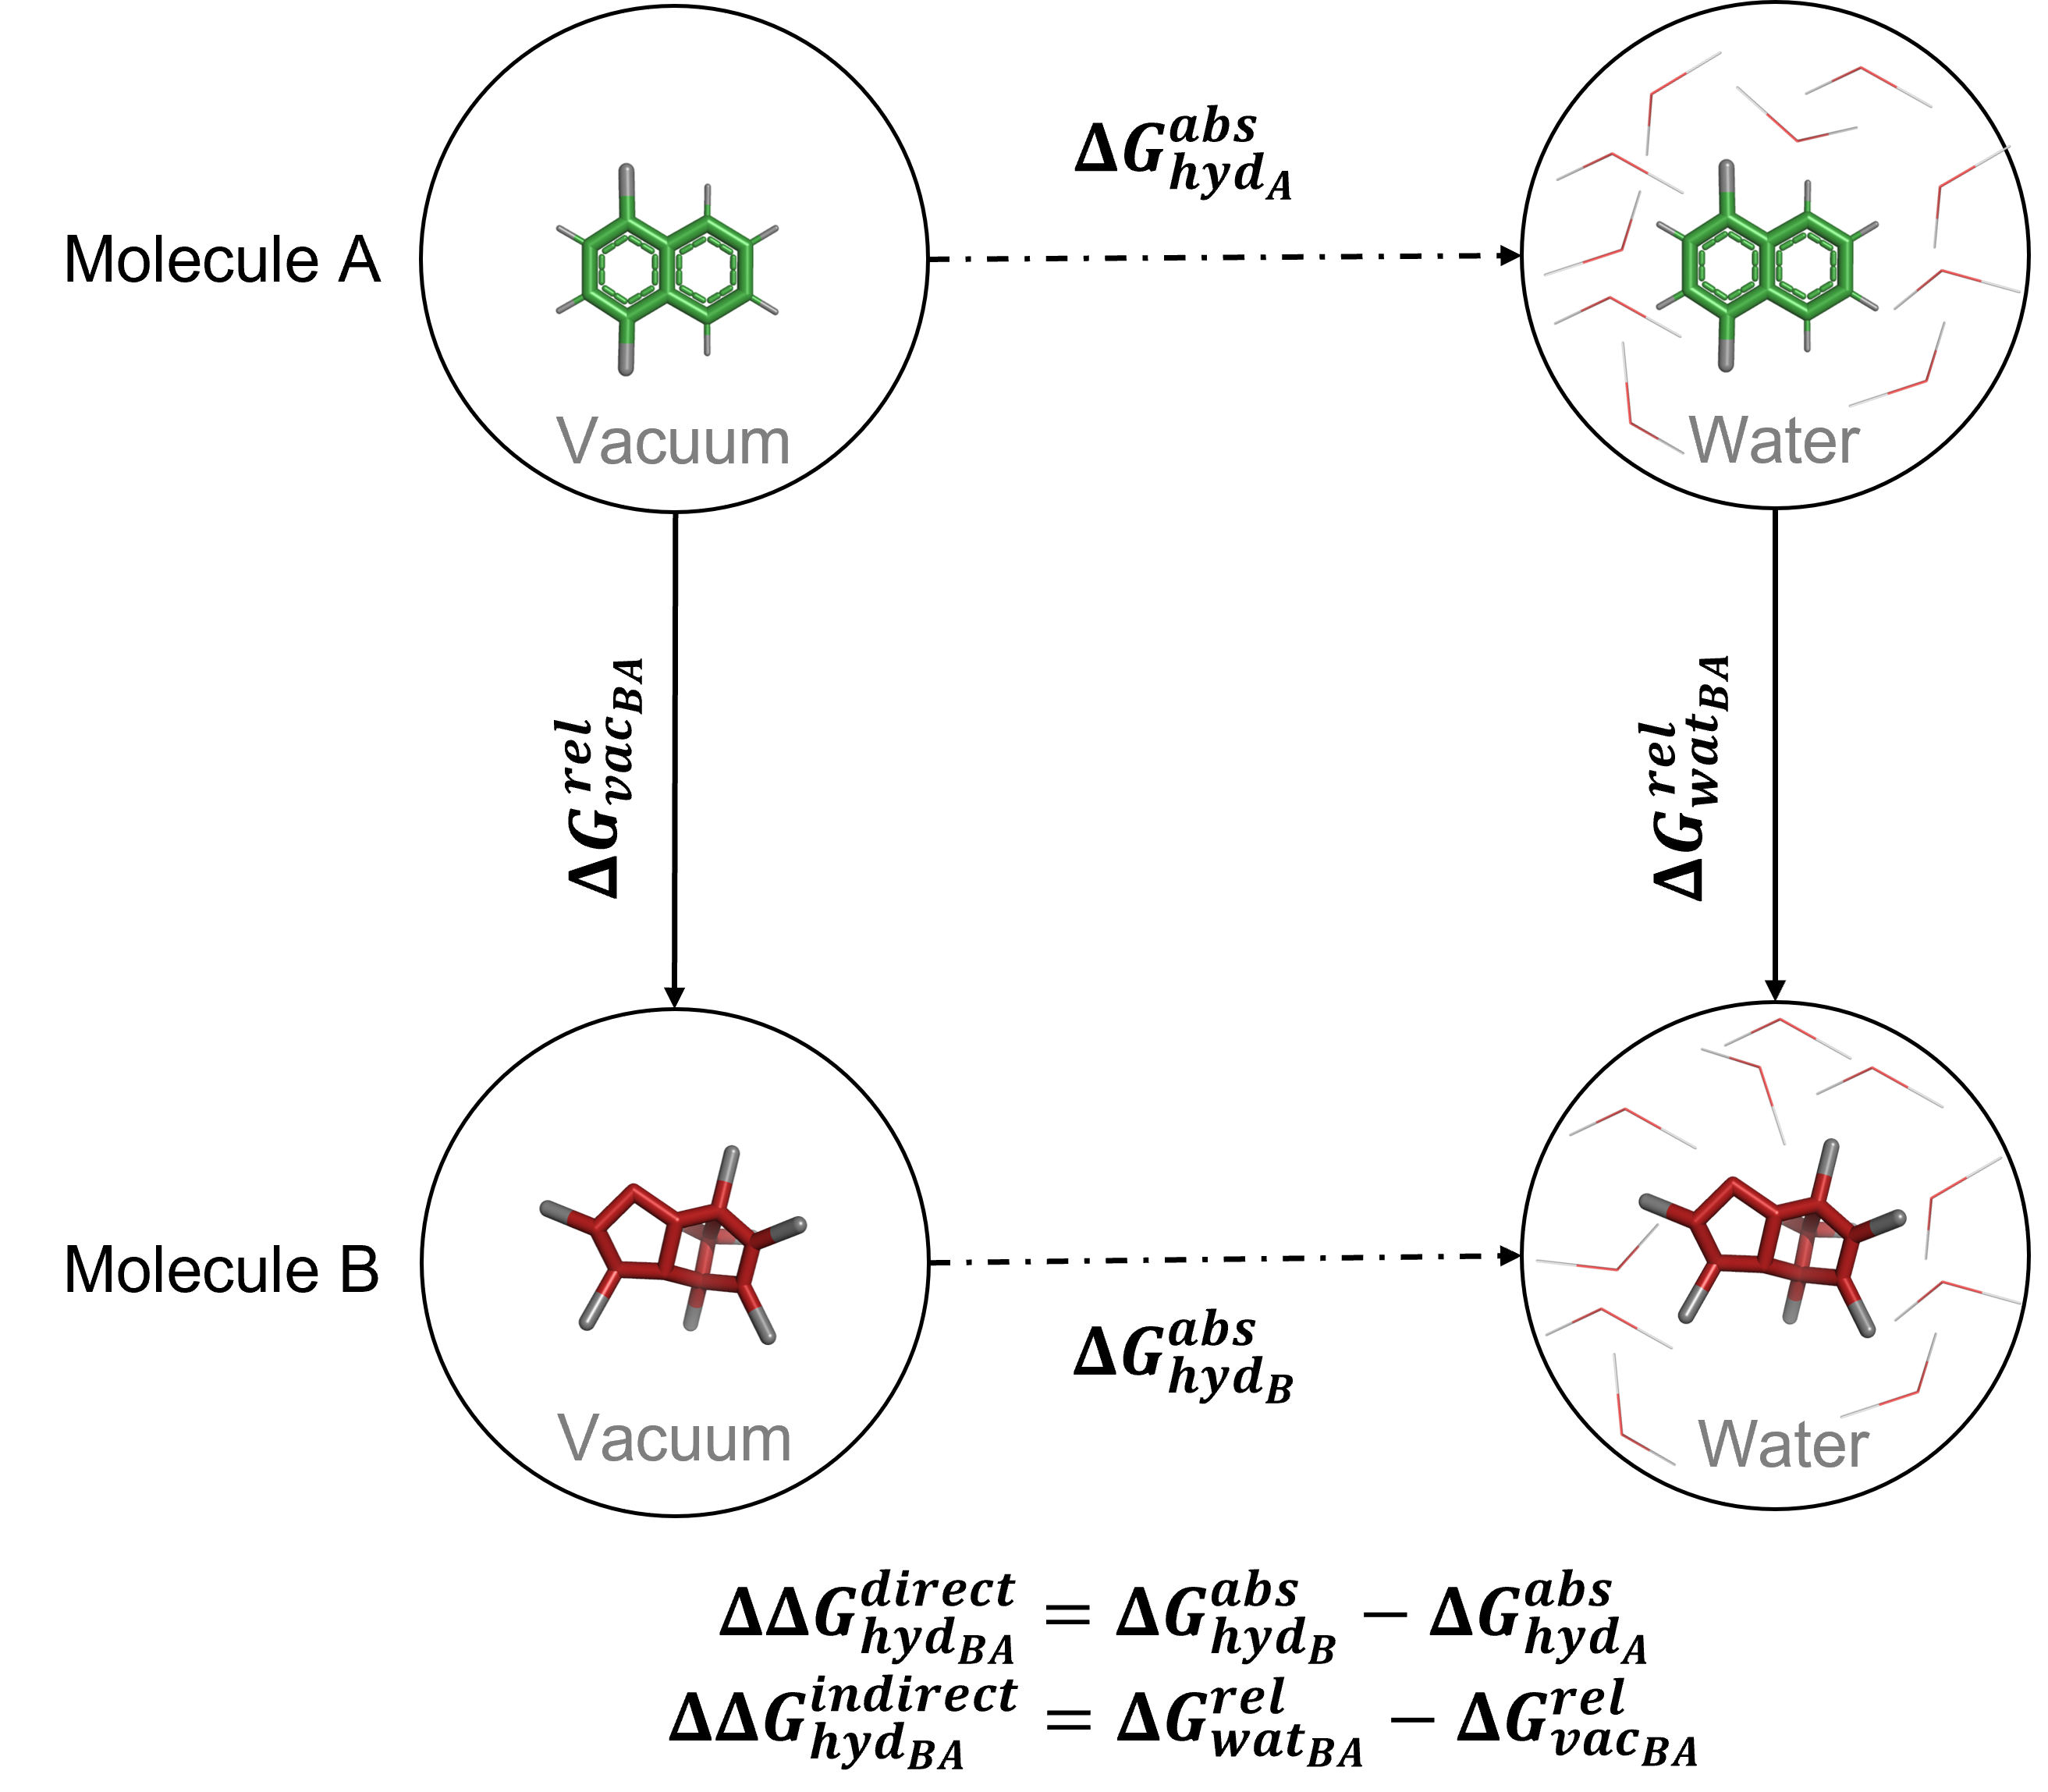
\includegraphics[width=0.8\textwidth]{fig/theory/ThermCycle.png}
    \caption{Thermodynamic cycle for the calculation of relative hydration free energies $\Delta \Delta G_{\text{hyd}_{AB}}$. The direct way to obtain $\Delta \Delta G_{\text{hyd}_{AB}}$ employs two absolute free-energy calculations giving $\Delta G^\text{abs}_{\text{hyd}_A}$ and $\Delta G^\text{abs}_{\text{hyd}_B}$. The indirect way uses two alchemical or relative free-energy calculations giving $\Delta G^\text{rel}_{\text{vac}_{AB}}$ and $\Delta G^\text{rel}_{\text{wat}_{AB}}$.
    }
    \label{fig:thermodynamic_cycle}
\end{figure}

\begin{table}[H]
\caption{Identifier of the ATB server\cite{Stroet2018}, IUPAC name, and canonical SMILES for the 16 molecules with experimental hydration free energies.}\label{tab:SI_moleculelist}
%\scriptsize
\resizebox{\columnwidth}{!}{%
\centering
\begin{tabular}{l | l | l }
Ligand & Identifier & IUPAC name \\
\hline
1 & \_O6T & 1,2-dimethoxybenzene \\
2 & \_O70 & (2R,5R)-2-methyl-5-prop-1-en-2-ylcyclohexan-1-one\\
3 & \_O71 & (1S,5R)-2-methyl-5-prop-1-en-2-ylcyclohex-2-en-1-ol \\ 
4 & \_P8I & cyclopentanone \\
5 & 6J29 & 1-amino-4-hydroxyanthracene-9,10-dione \\
6 & 6KET & 3-methoxyphenol \\
7 & 8018 & (1R,2S,3R,4R,6S,7S)-1,3,4,7,8,9,10,10-octachlorotricyclo[5.2.1.02,6]dec-8-ene \\
8 & E1VB & [1,2,2-Trifluoroethoxy]benzene\\
9 & F313 & 4-methoxyaniline \\
10 & G078 & 1,4-dimethylnaphthalene \\
11 & G277 & cyclohexa-2,5-diene-1,4-dione\\
12 & M030 & 1,3,5-trimethylbenzene \\
13 & M097 & 2-chloroaniline \\
14 & M218 & N-methylaniline \\
15 & S002 & bromomethylbenzene \\
16 & TVVS & pyridine-4-carbaldehyde\\
\end{tabular}
}
\end{table}


Pairwise TI calculations were carried out with a linked dual topology approach for the 16 molecules in a star-like scheme with molecule \textbf{12} as center, resulting in 15 relative hydration free energies (Figure \ref{fig: Pairwise_TI_M030_Graph}).
\begin{figure}[h]
    \centering
    
\includegraphics[width=\textwidth]{fig/methods/StateGraph_TI_2D_enumerated.png}
    \caption{Set of 16 molecules with experimental hydration free energies available \cite{Stroet2018,Wolfenden1987,Rizzo2006,Nicholls2008,Guthrie2009,Guthrie2014,Mobley2014}. The black lines indicate the pairs of molecules for which TI calculations were performed. RestraintMaker was used to select pairwise distance restraints between the central molecule and all others.} 
    \label{fig: Pairwise_TI_M030_Graph}
\end{figure}

\subsection{Simulation Details}
All simulations were carried out using the MD software package GROMOS\cite{Schmid2012} version 1.5.0 (freely available on \textit{http://www.gromos.net}),\cite{Ries2021B} the Python RE-EDS pipeline\\ (\textit{https://github.com/rinikerlab/reeds}) 
and PyGromosTools\cite{Lehner2021}\\ (\textit{https://github.com/rinikerlab/PyGromosTools}). 

In order to compare our results with the absolute hydration free energies reported in the ATB server,\cite{Stroet2018} the same simulation setup was used.
The simple point-charge (SPC) model\cite{Berendsen1981} was employed for water. A single cutoff radius of $1.2$~nm was used for the calculation of the non-bonded interactions. The integration time step was set to $2$~fs and the pairlist was updated every five steps. Long-range nonbonded interactions were calculated using a reaction-field correction\cite{Tironi1995} with $\varepsilon_{\text{rf}}=1$ for the simulations in vacuum and $\varepsilon_{\text{rf}}=61$ for the simulations in water.\cite{Heinz2001} The force constant for the distance restraints was set to $5000$ kJ$/($mol$\cdot$nm$^2)$.

\subsubsection{Thermodynamic Integration}
The topologies and coordinate files of the single states were obtained from the ATB server\cite{Stroet2018} and were merged to pairs using PyGromosTools\cite{Lehner2021}. 
The coordinates of the different single molecules were aligned to each other using the common molecular skeleton of the molecules (only rings), with the \textit{align} function in RDKit\cite{Landrum2021}. After the alignment, RestraintMaker was used to place four restraints with $d_\text{res} = 0.1$~nm (Figures \ref{SIfig: Pairwise_TI_M030_Graph} and \ref{SIfig:Pairwise_TI_AddRE-EDS_Graph}). 

\begin{figure}[H]
    \centering
    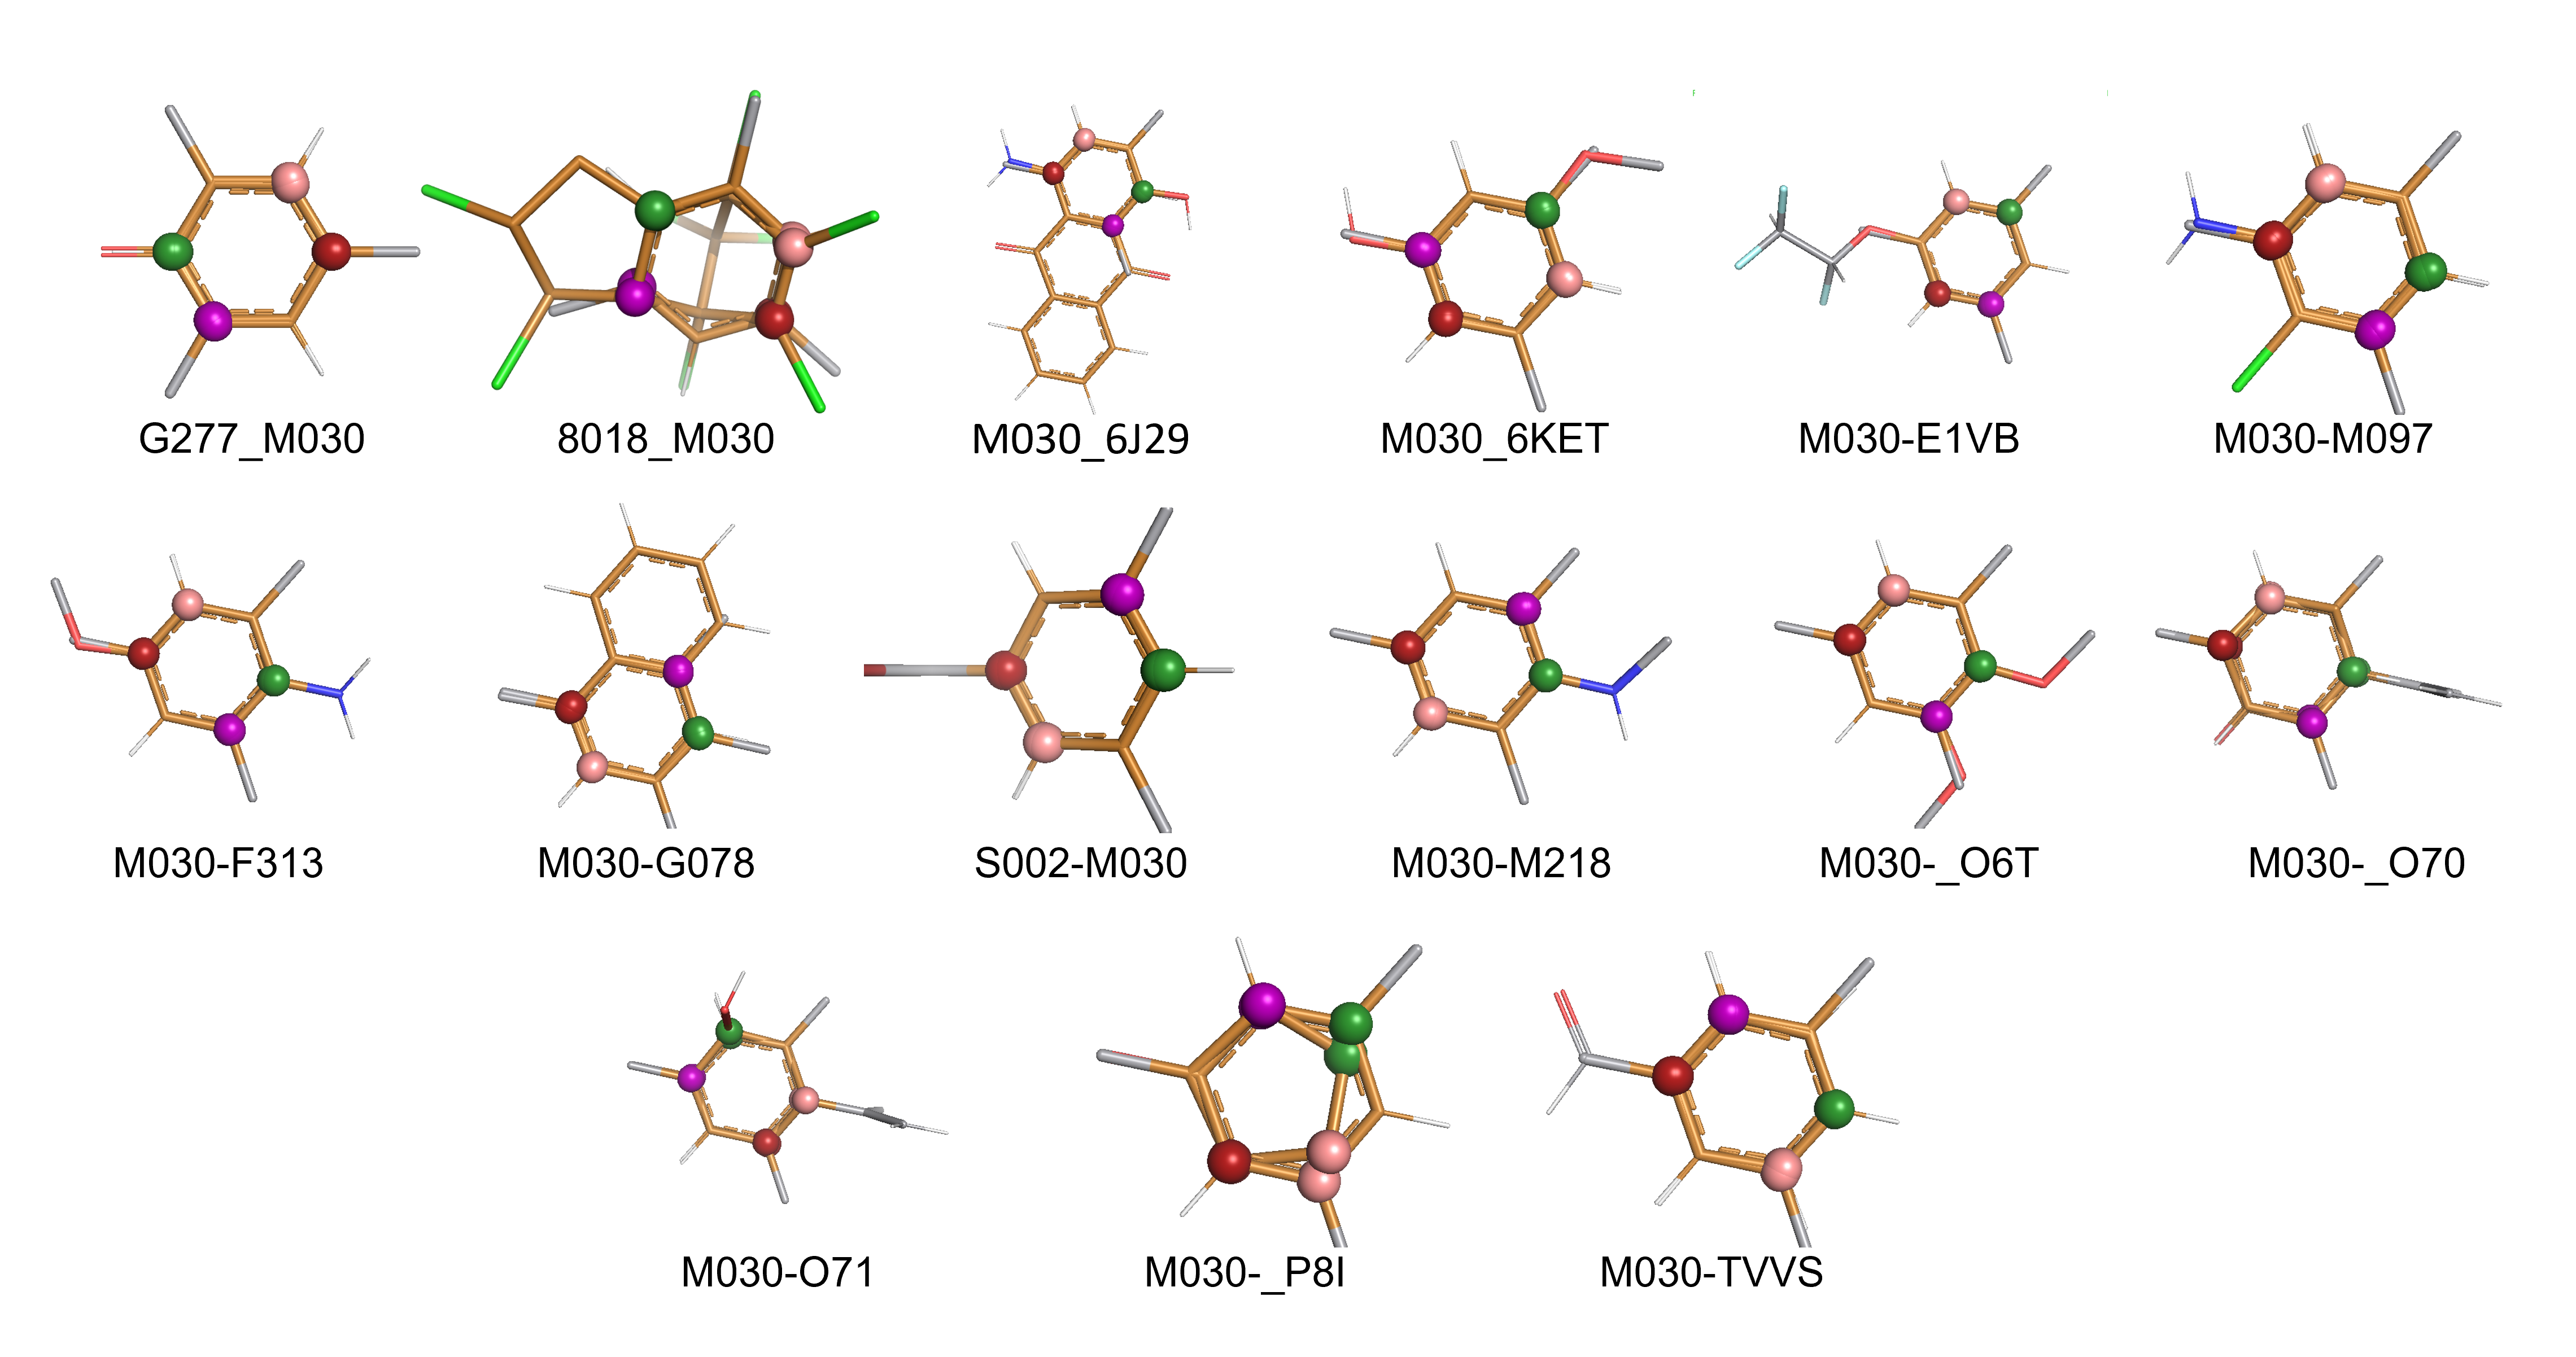
\includegraphics[width=\textwidth]{fig/results/pairwise/restraintPlacement/Restraints_PairwiseTI_M030Graph.png}
    \caption{Selected distance restraints (colored spheres) for the 15 pairwise TI calculations with molecule 12 (i.e. 1,3,5-timethylbenzene) as the central molecule (Figure \ref{fig: Pairwise_TI_M030_Graph}). For each pair, four distance restraints were determined with the greedy algorithm.}
    \label{SIfig: Pairwise_TI_M030_Graph}
\end{figure}


The computational boxes for the simulations in water were generated with the GROMOS++ \cite{Eichenberger2011} program \textit{simbox} using a minimal solute-to-wall distance of $0.8~$nm, and relaxed by energy minimization. The scripts can be found in the example folder on Github (\textit{https://github.com/rinikerlab/restraintmaker/tree/main/examples/publication/\\b\_ATB\_solvationFreeEnergies}).
The TI calculations were carried out with 21 evenly spaced $\lambda$-points between 0 and 1, both for the molecules in water and in vacuum. Each $\lambda$-point was equilibrated for $1$~ns, followed by a production run of $5$~ns. The free-energy differences were calculated using the Simpson integration implemented in the SciPy library.\cite{Virtanen2020}

\subsection{Analysis}
The analysis of the simulations was carried using GROMOS++ \cite{Eichenberger2011} and PyGromosTools \cite{Lehner2021}. In addition, the following Python packages were employed for the statistical analysis and plotting: Pandas \cite{Mckinney2010}, Matplotlib \cite{Hunter2007}, NumPy \cite{Vanderwalt2011}, SciPy \cite{Virtanen2020}, mpmath \cite{Johansson2013}, and Jupyter notebooks.\cite{Kluyver2016}
